\chapter{Generation, control and detection of 3D vortex structures in superfluid systems}
\label{ch:vortex_states}

In this chapter, I will discuss another application of the GPUE codebase, this time to the controlled creation of vortex structures in three dimensions with artificial magnetic fields generated by an optical nanofiber.
To the best of my knowledge, this is the first time an experimentally realizable protocol to generate vortex ring-like structures with a dielectric system has been suggested and investigated, and I also provide a method to detect whether a vortex ring is present in an elliptic-toroidal condensate.
This project encompasses three-dimensional vortices and coupled light-matter systems, so to begin, I will briefly discuss vortices in three-dimensional systems, followed by the model used for this project, where I will describe how the light from an optical nanofiber can generate and control vortex structures in BEC systems.
As a note, even though vortex dynamics are not shown in this study, GPUE is also capable of simulating the evolution in three-dimensions, and potential applications of vortex ring dynamics will be discussed in this chapter.
The contents of this chapter have recently been submitted to Phys. Rev. Fluids (arXiv:1910.02364)~\cite{schloss2019}.
In this study, I performed all simulations, with exception of vortex states generated in Figures~\ref{fig:VortexRings} and \ref{fig:HE21_3d}, which were performed under my supervision by Peter Barnett.
Figure~\ref{fig:mode_plot} was generated by multiple sources~\cite{nieddu2016, kumar2015}.
I also designed the GPUE codebase to allow for these simulations and visualized all data.
This project was supervised overall by Thomas Busch and Rashi Sachdeva.


\section{Three-dimensional vortex structures}
\label{sec:vortex}

As mentioned in Chapter~\ref{ch:splitop}, in BEC systems with large amounts of angular momentum and a single axis of rotation, the vortices will create a triangular, Abrikosov lattice~\cite{abo2001, abrikosov1957}. 
This regular structure is a direct consequence of the quantization of angular momentum in quantum mechanics, and in Chapter~\ref{ch:2d}, I discussed a small vortex lattice in two-dimensions by integrating out the $\hat z$ direction.
In this chapter, I will discuss fully three-dimensional vortex structures in BEC systems. 
In three dimensions, BEC systems have been shown to support a large variety of flow-related excitations, such as vortex lines and rings~\cite{madison2000,abo2001, wacks2014, anderson2001, bulgac2014, ku2016, matthews1999, yefsah2013}.
There are many interesting features to superfluid vortices in three dimensions, some of which follow from classical fluid dynamic theory~\cite{fetter2009}, which is a well-studied field and covered in many texts~\cite{faber1995, kundu2012, tritton1988, landau1987}.

By modifying the axis of rotation or inducing vorticity with either artificial magnetic fields or phase imprinting, one may create three-dimensional structures, like vortex rings.
Such structures are common when modelling large, three-dimensional superfluid systems and are a direct consequence of the required connections of vortex lines.
The stability of vortex rings is ensured by Kelvin's theorem~\cite{donnelly1991}, which means that unstable excitations may decay into vortex rings or objects with ring-like topology~\cite{anderson2001}.

In the case of multiple, interacting vortex rings, one can expect to find many similar features in superfluids to what has been found previously in classical, viscous fluids. 
If two vortex rings are generated in the same plane and in close proximity, it could be possible for the two velocity fields to interact, causing one ring to expand and slow down while the other contracts and speeds up. 
Under the right conditions, the lagging ring can pass the forward ring through a process known as \textit{leapfrogging}~\cite{sommerfield1950, caplan2014}.
This behavior can be extended to vortex ring bundles, in such systems the entire bundle will turn in on itself while moving in its self-induced velocity field~\cite{wacks2014}.

In addition to leapfrogging, vortex rings can interact through direct collisions~\cite{shariff1992}. 
In superfluid $^4$He, some of the earliest experiments on vortex collisions with vortex rings were performed by Schwarz in 1968~\cite{schwarz1968}.
In the case of a head-on collision, two identical, moving vortex rings will first grow in size before dispersing into a series of smaller vortex rings around their common circumference~\cite{lim1995}. 
These smaller rings are created by vortex reconnections, which can occur any time vortex lines are facing anti-parallel directions and it is energetically favorable to do so.

Finally, I will briefly discuss vortex reconnections, themselves.
As predicted by Feynman in 1955, vortex reconnections in a dissipative superfluid systems lead to larger vortices continually reconnecting into smaller ones until the loops become small enough to decay from dissipation or from interactions with boundaries~\cite{feynman1955}.
These reconnections produce sound waves when vortices directly interact and Kelvin waves when vortices indirectly interact~\cite{paoletti2011}.
When a vortex ring structure is not pinned by either gauge fields or rotation, it will evolve naturally by reconnecting into smaller and smaller vortex rings when in a turbulent system~\cite{jackson1999}. 
This means that one would expect to see vortex reconnections in any sufficiently complicated vortex tangle~\cite{barenghi2014}.

Though these dynamics are expected in superfluid systems, it is difficult to devise experimental systems that systematically generate the desired behavior.
In practice, complex three-dimensional structures cannot be easily created by stirring or rotating a BEC because vortex lines generated in this way must follow the axis of rotation, thus even simple vortex rings can be a challenge to create, control, and detect experimentally.
In most cases, including in most theoretical proposals, vortex ring generation in BEC systems relies on dynamic processes that do not create eigenstates of the system, such as the decay of dark solitons in multicomponent condensates~\cite{anderson2001} with the snake instability~\cite{ruostekoski2001}, the collision of symmetric defects~\cite{ginsberg2005}, or direct density engineering~\cite{shomroni2009, ruostekoski2005}.
There are other theoretical proposals that consider interfering two BEC systems~\cite{jackson1999}, using Feschbach resonances~\cite{pinsker2013}, or phase imprinting methods~\cite{ruostekoski2001}.
As a note, in inhomogeniously trapped BEC systems, vortex ring structures are known to be unstable, which has led to difficulties in their experimental observation~\cite{abad2008}.
In addition, imaging techniques employed for BECs are not suited to identify whether three-dimensional vortex structures are present.

To consistently control and generate more complex three-dimensional structures, methods beyond rotation must be used, and there are only a few known experimental systems that can do so~\cite{anderson2001,yefsah2013}.
There is also a large amount of interest in generating more complicated vortex structures, such as vortex knots~\cite{maucher2016, kleckner2016, ricca1999}.
Artificial magnetic fields seem to be a promising method for the generation of complex three-dimensional vortex structures in BEC systems~\cite{duncan2019}, and in this chapter, I will present a method to generate vortex rings, ring-lattices, and other vortex structures in three dimensions by using the artificial magnetic field generated by an optical nanofiber.

\section{Controlled creation of three-dimensional vortex structures in Bose--Einstein condensates using artificial magnetic fields}

One method to create artificial magnetic fields involves the interaction between an atomic system in a dressed state and an electric field that is tuned near an atomic resonance frequency~\cite{dalibard2011}.
In practice, this means that one can create a configurable artificial magnetic field with an appropriately tuned electric field that varies strongly over short distances, such as those found in the near-field regime on the surface of a dielectric system when light undergoes total internal reflection~\cite{mochol2015}.
One such system that suits this purpose and can be used to generate vortex ring structures in BEC systems is the optical nanofiber, which has several propagation modes to facilitate the generation of configurable artificial magnetic fields.

Optical nanofiber systems can be created by heating and stretching optical fibers until their thinnest region is roughly hundreds of nanometers in diameter~\cite{ward2006, tong2003}.
At this scale, the wavelength of light is larger than the diameter of the fiber and the strength of the evanescent field is significantly enhanced~\cite{yariv1997}.
The form of the evanescent field varies greatly depending on the optical modes propagating through the nanofiber, and I will show that this can be used to generate interesting and tunable artificial magnetic fields.

Optical nanofibers are already used in many different experiments with ultracold atoms~\cite{vetsch2010, lacroute2012, nieddu2016, sague2007, russell2011, kumar2015}, and trapping potentials around 200nm from the fiber surface can be created with two differently detuned input fields~\cite{kien2004, phelan2013}.
Our proposed device will allow for the creation of vortex rings in BEC systems that are trapped toroidally around the nanofiber by coupling the BEC to the evanescent field created by different modes propagating through the nanofiber~\cite{sachdeva2017}.
A schematic of this system is depicted in Figure~\ref{fig:device}

\begin{figure}[t]
\begin{center}
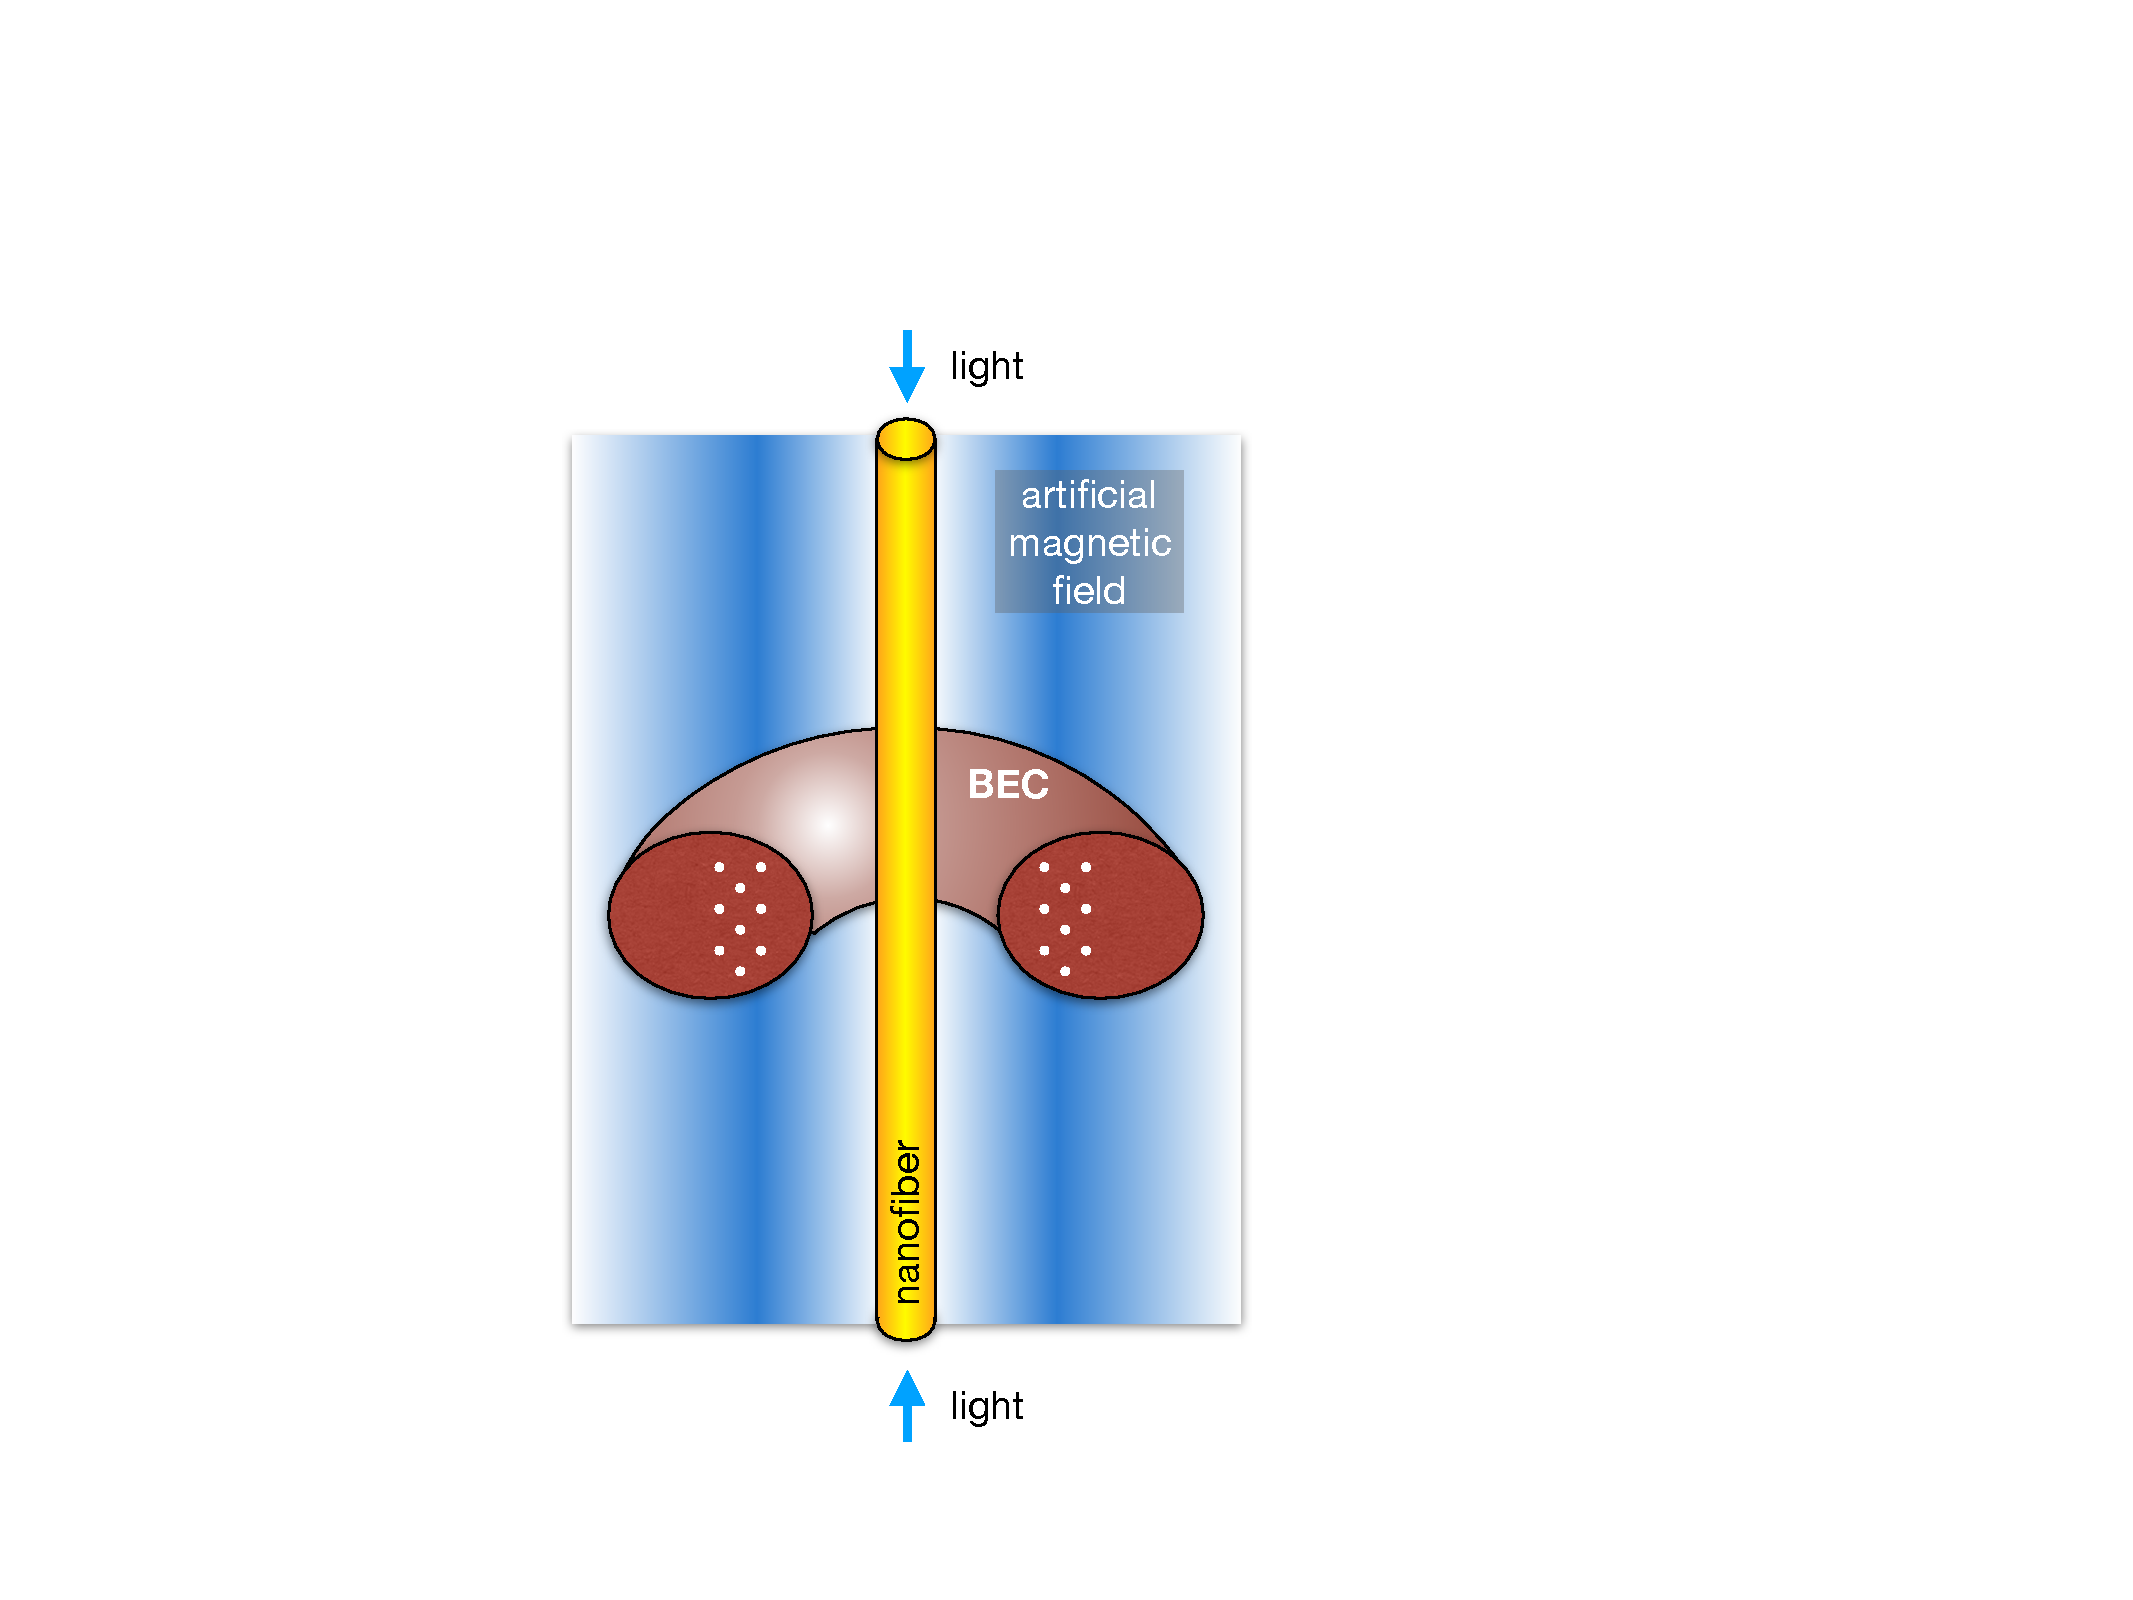
\includegraphics[width=0.4\textwidth]{data/3d/Schematic_TB}
\end{center}
\caption{Schematic of the system. Blue or red-detuned light is sent into the nanofiber (yellow), creating an evanescent field and artificial magnetic field (blue) that influences the BEC (maroon) held by a toroidal trapping potential. If the artificial magnetic field strength is greater than a threshold value, vortex rings (white) will appear and begin to arrange themselves into a triangular lattice.}
\label{fig:device}
\end{figure}

In this setup, it is also possible to detect whether a vortex ring is present in the system by exciting the scissors mode using an elliptic-toroidal trapping geometry~\cite{cozzini2003, guery1999, marago2000}.
This can be done by tilting the trap radially from the center of the torus, which will cause the BEC to oscillate in and out in the new potential, similar to the oscillation shown in Chapter~\ref{ch:splitop} for a simple harmonic oscillator.
Without a vortex present, this oscillation possesses a single frequency, whereas in the presence of a vortex ring, it will contain two frequencies that average to the vortex-less oscillation frequency, similar to scissors mode oscillations in a two-dimensional, elliptically-trapped BEC~\cite{smith2004, zambelli1998, stringari2001}.

\subsection{Bose--Einstein condensate dynamics in the presence of an optical nanofiber}

As discussed in Chapter~\ref{ch:splitop}, in the presence of an artificial magnetic field, the GPE becomes,

\begin{equation}
i\hbar \frac{\partial \Psi}{\partial t} = \left[\frac{(p-m\mathbf{A}({\bf r}))^2}{2m} + V_{\text{trap}}({\bf r}) + g|\Psi|^2 \right] \Psi.
\end{equation}

\noindent Here, all values are defined as before.
The artificial vector potential can take many forms, but for here, I will again choose a description based on Berry's connection~\cite{dalibard2011},

\begin{equation}
  \mathbf{A} = i\hbar \braket{\Psi_l | \nabla \Psi_l},
\end{equation}
\noindent where $\Psi_l$ is the atomic wavefunction in some dressed state $l$.

Considering a dressed, two-state atoms in the presence of an optical field, its states can be written within the rotating wave approximation as~\cite{mochol2015},
\begin{align}
\ket{\Psi_1({\bf r})} &= 
\begin{pmatrix}
    \cos[\Phi({\bf r})/2] \\
     \sin[\Phi({\bf r}) /2]e^{i\phi(z)} 
\end{pmatrix},\\
\ket{\Psi_2({\bf r})} &= 
\begin{pmatrix}
    -\sin[\Phi({\bf r}) /2]e^{-i\phi(z)} \\
    \quad\cos[\Phi({\bf r})/2]
\end{pmatrix},
\end{align}
\noindent where $\phi(z)$ is the phase of the optical field and $\Phi({\bf r}) = \arctan(|\kappa({\bf r})|/\Delta)$, with $\Delta = \omega_0 - \omega$ being the detuning and $\kappa({\bf r}) = \mathbf{d} \cdot \mathbf{E}({\bf r}) / \hbar$ being the Rabi frequency.
The atomic dipole moment is given by $\mathbf{d}$ and $\mathbf{E(\mathbf{r})}$ is the electric field.
Here the form of $\mathbf{A}$ follows the form of the optical fields, and the artificial magnetic field is given by $\mathbf{B}= \nabla \times \mathbf{A}$; therefore, it is possible to influence the magnetic field and vortex structures generated with this system by modifying the optical profile around the nanofiber.

For optical nanofibers, one can determine which modes will propagate in the system by calculating the $V$-number, with $V = k_0a\sqrt{n_1^2 - n_2^2}$, where $a$ is the fiber radius, $n_1$ is the refractive index of the fiber, $n_2$ is the refractive index of the cladding, and $k_0 = \omega/c$ with $\omega$ being the frequency of the input light beam.
The $V$ number can be controlled by modifying the radius of the fiber.
The way in which light propagates through the fiber for each mode is characterized by the modal propagation constant, $\beta$,
the effective refractive index of the fiber is $n_\text{eff} = \beta / \kappa_0$.
In Figure~\ref{fig:mode_plot}, a plot of $n_\text{eff}$ vs $V$ number is shown in (a) and it can be seen that certain modes cannot propagate until certain threshold values are reached.
In (b) and (c), the simulated and experimental images of the fiber output are shown for the LP$_{11}$ group, which is a combination of the HE$_{21\text{even}}$, HE$_{21\text{odd}}$, TE$_{01}$ and the TM$_{01}$ modes.
For the system considered in this chapter, the fiber has been tapered such that the cladding is the vacuum, itself, with $n_2=1$; therefore, higher order modes can only be sustained if $V > V_c \simeq 2.405$.
Below this value, only the fundamental mode can propagate in the system.

\begin{figure}

\center 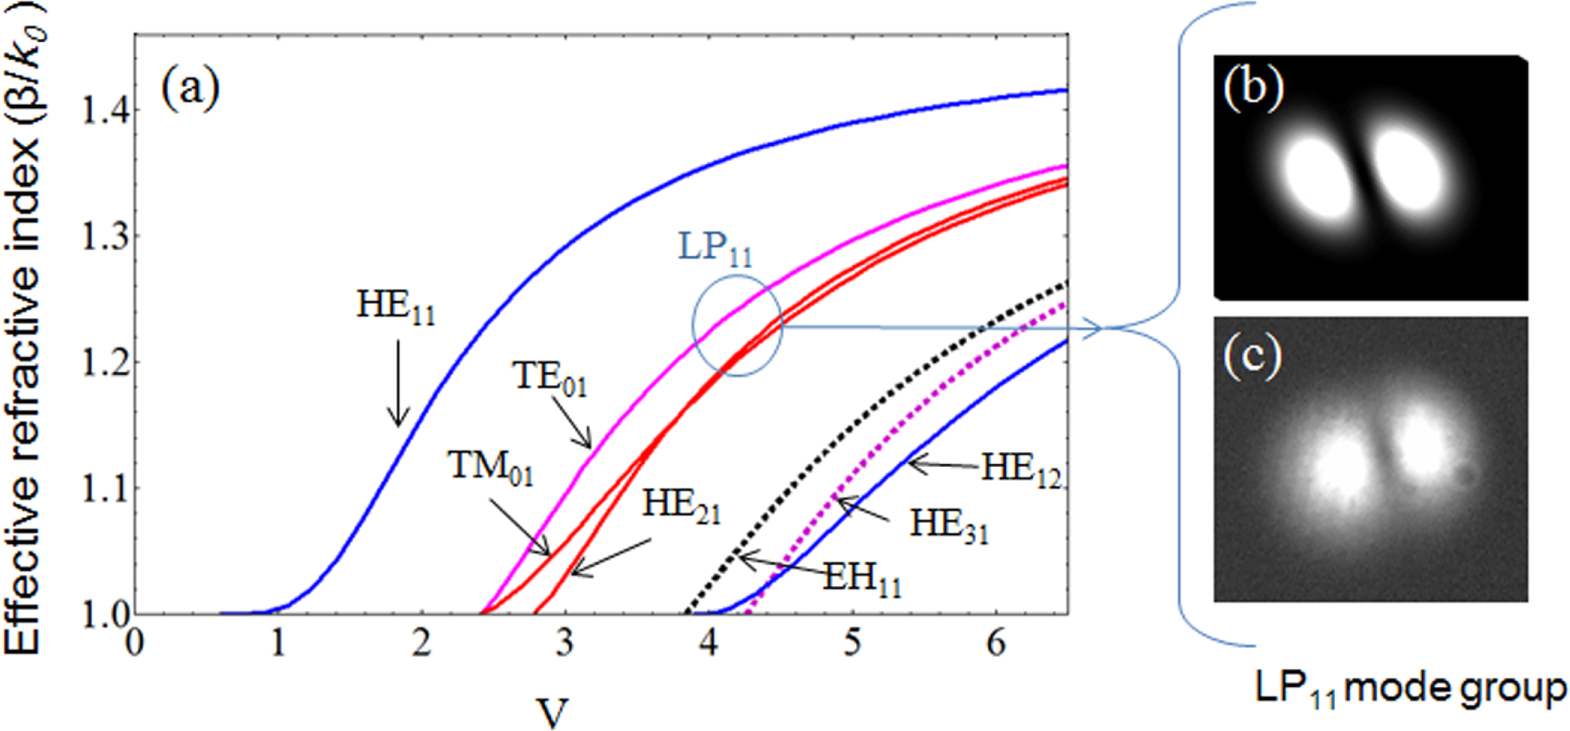
\includegraphics[width=\textwidth]{data/3d/fiber/mode_plot.jpg}
\caption{(a) Plot of effective refractive index and $V$ number of an optical fiber.
The circle indicates the LP$_{11}$ group, which is the first higher-order group composed of the HE$_{21\text{even}}$, HE$_{21\text{odd}}$, TE$_{01}$ and the TM$_{01}$ modes.
(b) Simulated and (c) experimental images of the output from the LP$_{11}$ group are also shown.
Reproduced from ~\cite{nieddu2016, kumar2015}.
}
\label{fig:mode_plot}
\end{figure}

Using cylindrical coordinates, the evanescent field of the HE$_{\ell m}$ mode with circular polarization is~\cite{minogin2010},

\begin{align}
        E_r &= iC[(1-s)K_{\ell-1}(qr) + (1+s)K_{\ell+1}(qr)]e^{i(\omega t- \beta z)}, \\
        E_\phi &= -C[(1-s)K_{\ell-1}(qr) - (1+s)K_{\ell+1}(qr)]e^{i(\omega t- \beta z)}, \\
        E_z &= 2C(q/\beta)K_\ell(qr)e^{i(\omega t - \beta z)},
\end{align}
where
\begin{align}
        s &= \frac{1/h^2a^2 + 1/q^2a^2}{J_\ell'(ha)/[haJ_\ell(ha)]+K_\ell'(qa)/[qaK_\ell(qa)]}, \\
        C &= \frac{\beta}{2q}\frac{J_\ell(ha)/K_\ell(qa)}{\sqrt{2\pi a^2(n_1^2N_1+n_2^2N_2)}},
\end{align}
and 
\begin{align}
N_1 =&\frac{\beta^2}{4h^2}\Big[(1-s)^2\left[J_{\ell-1}^2(ha)+J_\ell^2(ha)\right]\nonumber \\
   & \qquad+(1+s)^2\left[J_{\ell+1}^2(ha)-J_\ell(ha)J_{\ell+2}(ha)\right]\Big] \nonumber\\
   & +\frac12\left[J_\ell^2(ha) - J_{\ell-1}(ha)J_{\ell+1}(ha)\right], \\
N_2 =& \frac{J_\ell^2(ha)}{2K_\ell^2(qa)}\Bigg( \frac{\beta^2}{4q^2}\Big[(1-s)^2\left[K_{\ell-1}^2(qa)-K_\ell^2(qa)\right] \nonumber\\
   & \qquad\qquad\quad-(1+s)^2\left[K_{\ell+1}^2(qa)-K_\ell(qa)K_{\ell+2}(qa)\right]\Big] \nonumber\\
   & \qquad\qquad \left[K_\ell^2(qa) + K_{\ell-1}(qa)K_{\ell+1}(qa)\right]\Bigg ).
\end{align}
The mode geometry is given by $J_n(x)$, the Bessel function of the first kind, $K_n(x)$, the modified Bessel function of the second kind, and $\beta$, the propagation constant of the fiber.
The scaling factors are given by $q = \sqrt{\beta^2-n_2^2k_0^2}$ and $h = \sqrt{n_1^2k_0^2 - \beta^2}$, the normalization constant is $C$ and $s$ is a dimensionless parameter.

\begin{figure}[tb]
 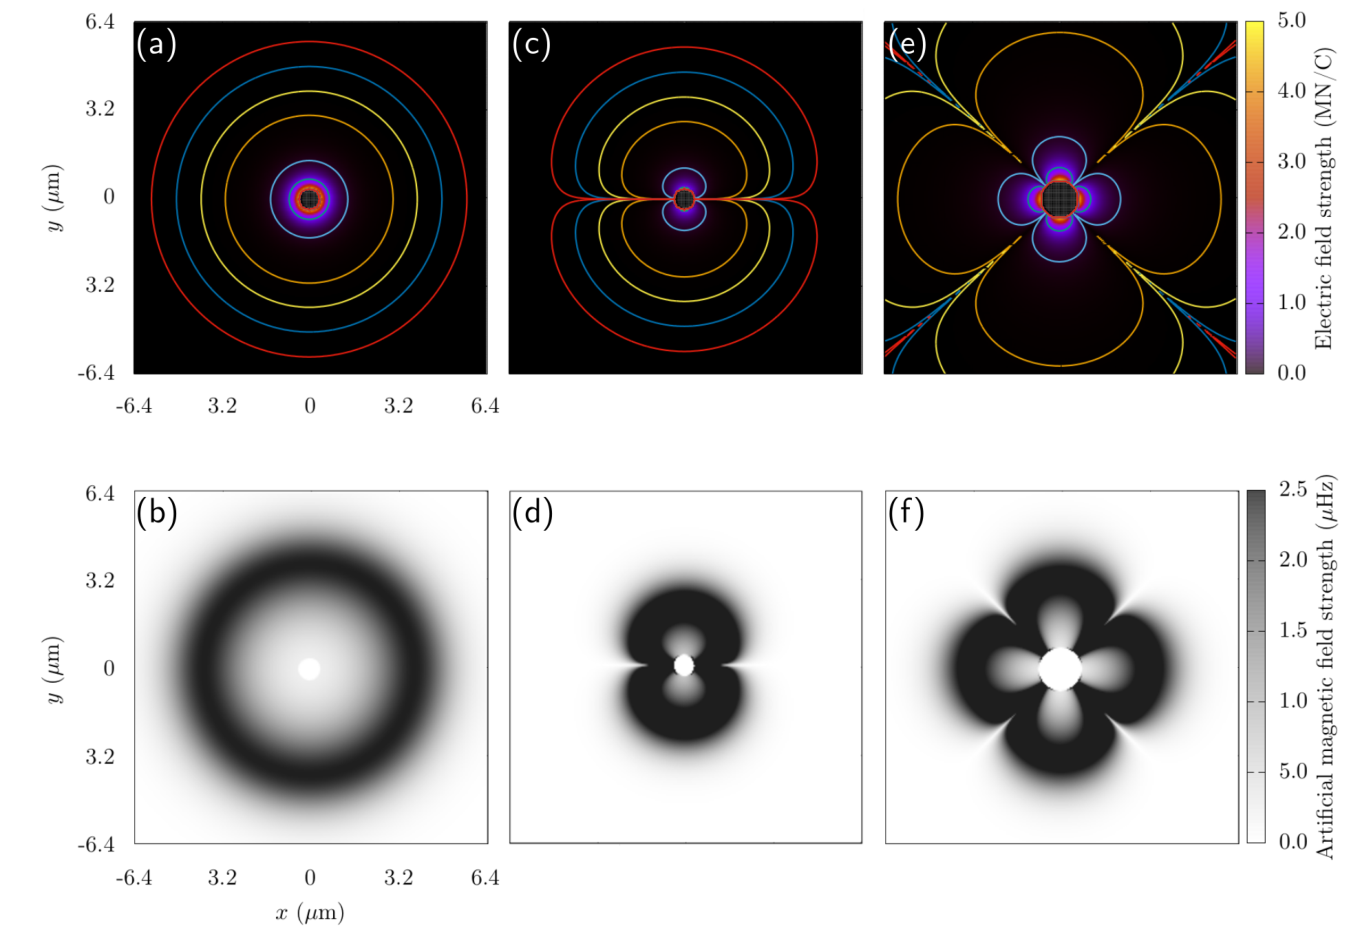
\includegraphics[width=\linewidth]{data/3d/all_fields.pdf}
         \caption{Images of electric and artificial magnetic field profiles for [(a) and (b)] the fundamental HE$_{11}$ mode with circular polarization, [(c) and (d)] the HE$_{11}$ mode with linear polarization, and [(e) and (f)] the HE$_{21}$ mode with linear polarization. For these calculations, the input power is 372~nW in (a) and (b) , 16~nW in (c) and (d), and 418~nW in (e) and (f). For the HE$_{11}$ mode, the nanofiber radius is 200~nm with blue-detuned light of 700~nm, and for the HE$_{21}$ mode, the nanofiber radius is 400~nm with red-detuned light of 980~nm}
 \label{fig:EtoB}
\end{figure}

When the input light field is linearly polarized, it is convenient to write the  Cartesian components of the evanescent electric field as 
\begin{align}
E_x =& \sqrt 2 C\Big[(1-s)K_{\ell-1}(qr)\cos(\phi_0)
      +(1+s)K_{\ell+1}(qr)\cos(2\phi-\phi_0)\Big]e^{i(\omega t - \beta z)}, \\
E_y =&\sqrt 2 C\Big[(1-s)K_{\ell-1}(qr)\sin(\phi_0)
      +(1+s)K_{\ell+1}(qr)\sin(2\phi-\phi_0)\Big]e^{i(\omega t - \beta z)}, \\
E_z = & 2\sqrt 2 i C(q/\beta)K_\ell(qr)\cos(\phi - \phi_0)e^{i(\omega t - \beta z)}.
\end{align}
Here $\phi_0$ determines the orientation of polarization, with $\phi_0 = 0$ being along the $x$ axis and $\pi/2$ being along the $y$ axis.
The artificial vector potential produced by such evanescent fields around an optical nanofiber is then given by \cite{sachdeva2017}
\begin{equation}
\mathbf{A} = \hat{z} \hbar \kappa_0 (n_1 + 1) \tilde{s} \left[\frac{|d_rE_r + d_{\phi}E_{\phi} + d_zE_z|^2}{1 + \tilde s^2|d_rE_r + d_{\phi}E_{\phi} + d_zE_z|^2} \right],
\end{equation}
where $\tilde s = \frac{|\mathbf{d}\cdot\mathbf{E}|}{\hbar |\Delta|}$ and
the corresponding magnetic field $\mathbf{B} = \nabla \times \mathbf{A}$ can be calculated to be
\begin{align}
\mathbf{B} =& \frac{\hbar \kappa_0 s^2(n_1 + 1)}{(1+\tilde s^2|d_rE_r + d_{\phi}E_{\phi} + d_zE_z|^2)^2} \nonumber\\
&\times \bigg[ \hat\phi  \frac{\partial}{\partial r} |d_rE_r + d_{\phi}E_{\phi} + d_zE_z|^2 \nonumber\\
&\qquad- \hat r \frac{1}{r} \frac{\partial}{\partial \phi} |d_rE_r + d_{\phi}E_{\phi} + d_zE_z|^2 \bigg ].
\end{align}
This shows that the $\mathbf{B}$ field has only components in the $\hat \phi$ and $\hat r$ directions, which means that all field lines lie in the horizontal plane if the fiber is aligned along the vertical $\hat z$ direction.

This also means that a BEC trapped toroidally around the nanofiber would facilitate vortex structures that wrap around the nanofiber and potentially close on themselves in the form of vortex rings; however, other vortex structures are possible as well.
In addition, the value of $\tilde s$ governs the amplitude and range of the magnetic field, and as such, it is possible to manipulate the size and shape of the generated vortex rings by changing the detuning and intensity of the electric field~\cite{sachdeva2017}.

To investigate the fundamental properties of this system, I will consider the fundamental HE$_{11}$ mode with circular polarization, the HE$_{11}$ mode with linear polarization, and the HE$_{21}$ mode with linear polarization.
Though even higher-order modes may be generated by the optical nanofiber, increasing the $V$-number to facilitate these modes also requires increasing the fiber radius and therefore introducing instabilities and more coupling processes.
It is also possible to create even more complex field configurations by interfering different modes.
The electric field configurations and their corresponding magnetic field profiles can be seen in Figure~\ref{fig:EtoB}.
Here, the circularly polarized HE$_{11}$ mode will create a cyllindrically symmetric electric (a) and magnetic (b) field profiles; however, linearly polarized light will create a lobed structure for both (c and d).
When using the linearly-polarized HE$_{21}$ mode, four petals appear in the electric and magnetic field profiles, which suggest unusual vortex structures.
Now I will discuss what types of vortex structures can be generated with this system, including the possibility of generating vortex ring lattices.

\subsection{Ground state vortex configurations}

\begin{figure}[tb]
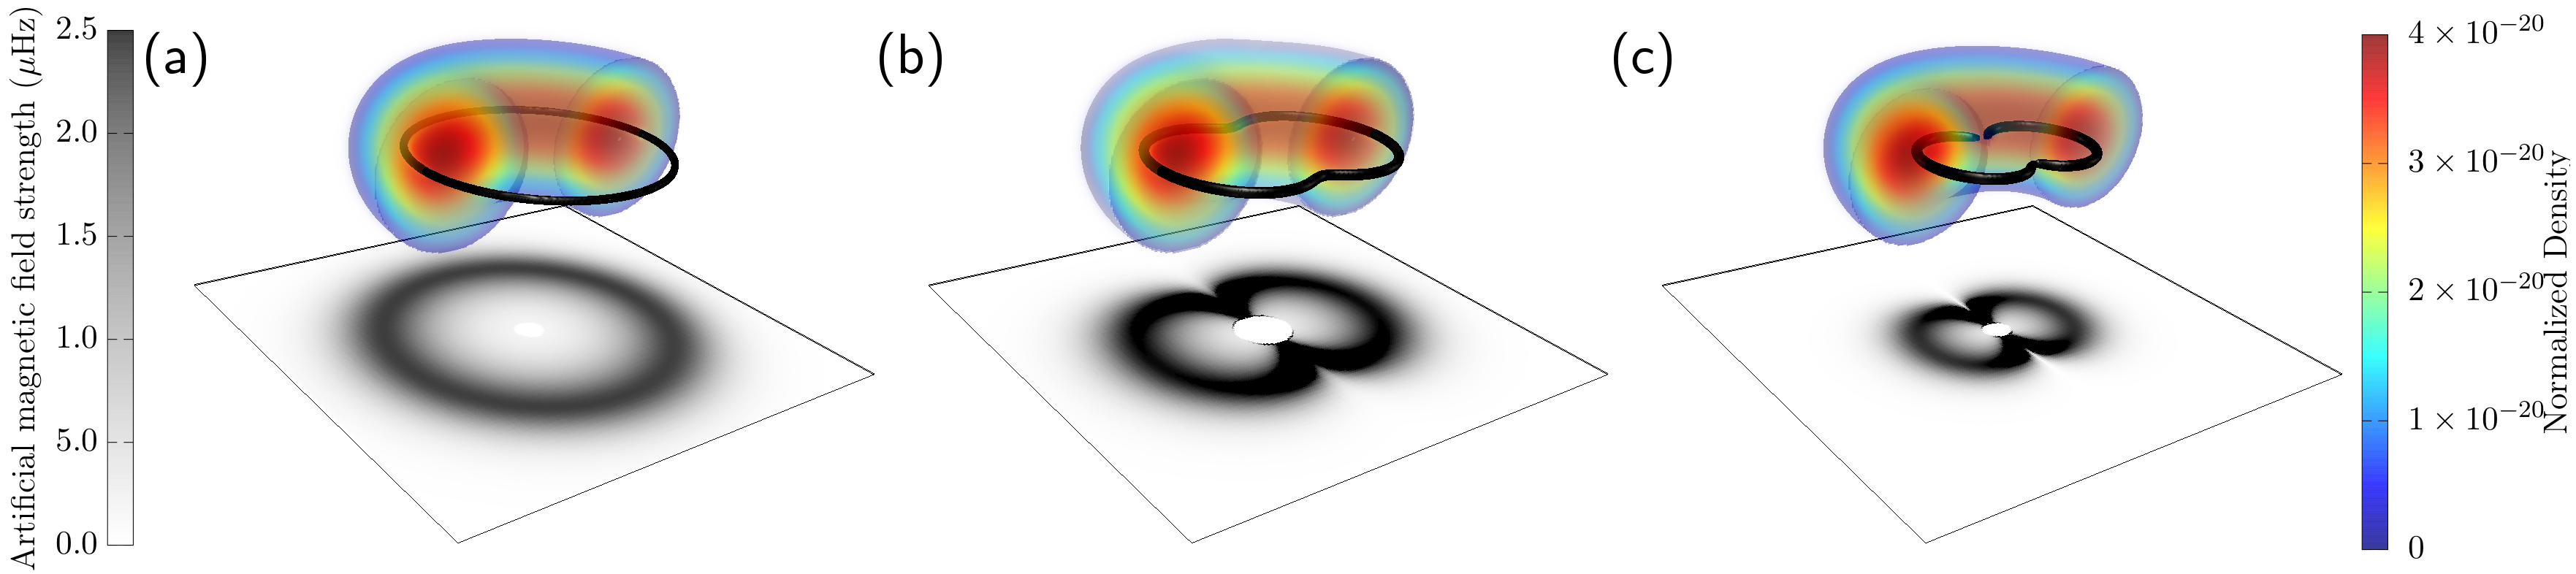
\includegraphics[width=\textwidth]{data/3d/vortex_transition.png}
\caption{Vortex configurations for different magnetic field profiles from the nanofiber for the fundamental HE$_{11}$ mode with (a) circular polarization, (b) elliptical polarization, and (c) linear polarization along the $\hat y$ direction.
The vortex distributions have been found via an isosurface on the Sobel filtered wavefunction density for a $^{87}$Rb BEC and all optical fiber fields are normalized and for a nanofiber of 200~nm in radius with blue-detuned light of 700nm.
The magnetic field profiles shown in the shaded region beneath wavefunction density are similar to those in Figure~\ref{fig:EtoB}(b) and (d).}
\label{fig:VortexRings}
\end{figure}

We will use GPUE~\cite{schloss2018} to describe a $^{87}$Rb condensate with $1\times10^5$ atoms with a scattering length of $a_s=4.76 \times 10^{-9}$ m on a three-dimensional grid of $256^3$ points with a spatial resolution of 50 nm.
We assume a toroidal trapping potential around the fiber given by,
\begin{equation}
V_\text{trap} = m(\omega_r^2(r-\eta)^2 + \omega_z^2z^2),
\label{eqn:potential}
\end{equation}

\noindent where the frequencies in the $\hat r$ and $\hat z$ directions are chosen to be $\omega_r = \omega_z = 7071$Hz to match typical experimental conditions in fiber trapping \cite{vetsch2010}.
Here, $\eta$ describes the distance of the center of the torus from the center of the fiber and is chosen such that the atoms are trapped beyond the van-der-Waals potential of the fiber.
For the HE$_{11}$ mode, the fiber radius is 200\,nm and $\eta = 3.20$\,$\mu$m, creating a toroidal BEC with an inner radius of roughly 300\,nm from the fiber surface.
For the HE$_{21}$ mode, the fiber radius is increased to 400 nm, but all other parameters are kept the same, creating a toroidal BEC with an inner radius of roughly 150 nm.

\begin{figure}[tb]
\center 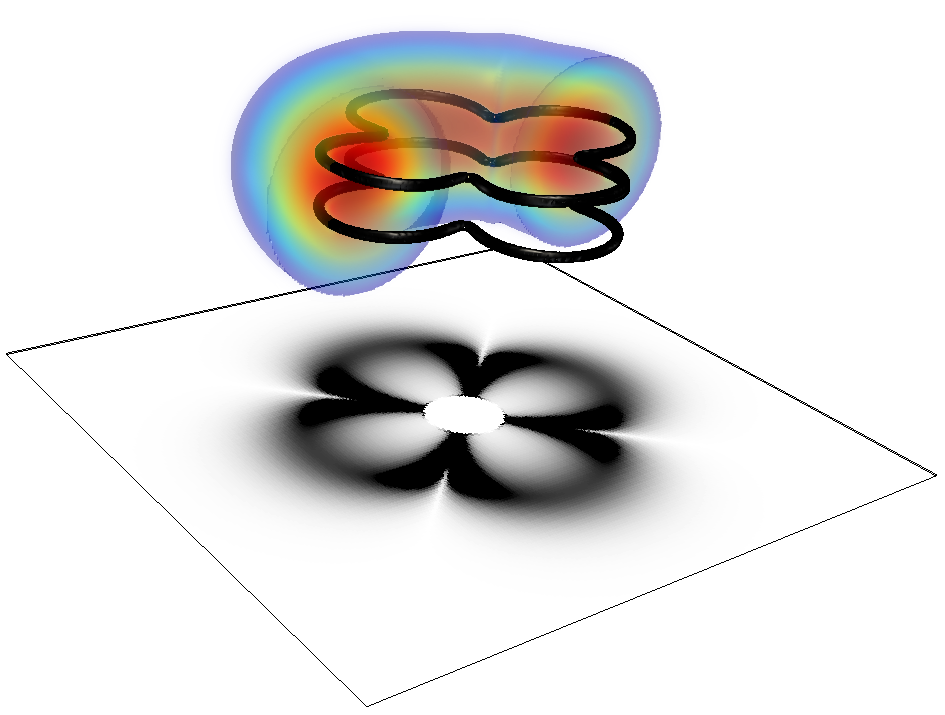
\includegraphics[width=0.5\linewidth]{data/3d/HE21_3d.png}
 
 \caption{Vortex configuration for the HE$_{21}$ mode with linear polarization along the $\hat y$ direction.
\label{eqn:potential}
The magnetic field profile is similar to the one shown in Figure~\ref{fig:EtoB}(f), and has been calculated for a nanofiber of 400~nm in radius with red-detuned light of 980~nm.}
 \label{fig:HE21_3d}
\end{figure}

As shown in Figure~\ref{fig:VortexRings}(a), when simulating the HE$_{11}$ mode with these parameters, a single vortex line appears that wraps around the fiber and reconnects in the form of a single vortex ring as the ground state solution.
In contrast, the linearly polarized HE$_{11}$ mode in Figure~\ref{fig:VortexRings}(c) shows a ground state where the vortex line bends toward the center of the torus, creating two vortex lobes.
As a note, the vortex lines do not follow the magnetic field lines exactly, but instead reconnect to the neighboring lobe when approaching each other within a healing length.
If elliptically polarized light is considered, one can see a hybrid ground state between the circularly and linearly polarized modes, shown in Figure~\ref{fig:VortexRings}(b).
Finally, I show a four-petal ground-state solution when using the HE$_{21}$ linearly polarized mode in Figure~\ref{fig:HE21_3d}.
Here, I also show that it is possible to generate multiple vortex structures in-line with themselves by increasing the intensity of the artificial magnetic field.

\begin{figure}
\center 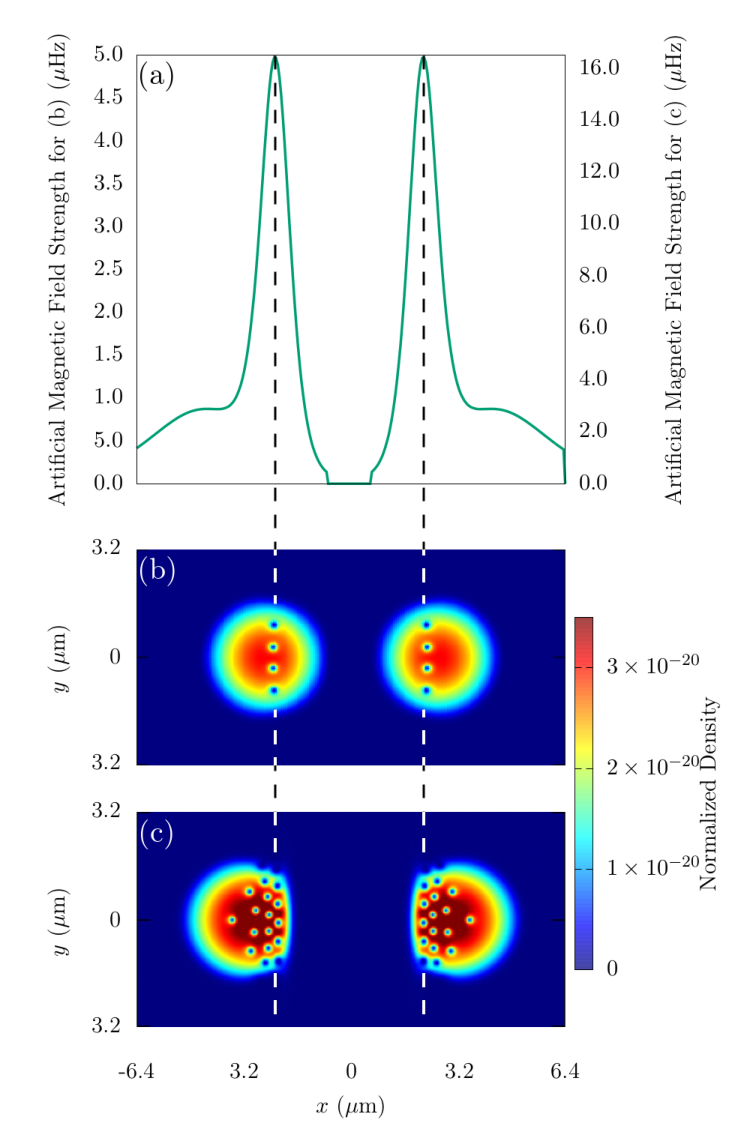
\includegraphics[width=0.8\linewidth]{data/3d/vortex_line_all.pdf}
\caption{(a) The magnetic field profile along the $x$-direction for the fundamental HE$_{11}$ mode with circular polarization outside a fiber of 200~nm radius.
Note that for this mode and polarization the whole system is azimuthally symmetric.
For weak fields (see (b)) this leads to a small number of vortices that align along the line at which the magnetic field is maximal and for larger fields (see (c)) more vortex rings appear that form the beginning of an Abrikosov lattice.
The optical fiber field and wavefunction density have been normalized and are for a nanofiber of 200~nm in diameter with blue-detuned light of 700nm and a $^{87}$Rb BEC respectively.}
\label{fig:field_triangular}
\end{figure}

This indicates that it is possible to generate interesting vortex ring lattice structures in three-dimensions by sufficiently increasing the complexity of the artificial magnetic field.
To study the control of multiple vortex structures with this system, I first simulated a system with low artificial magnetic field strength and showed that this simulation will cause all vortex rings to line up at peaks in the magnetic field in Figure~\ref{fig:field_triangular}(a and b).
As the magnetic field is increased from this point, the vortex rings begin to pack together and form an Abrikosov-like lattice in-line with peaks in the artificial magnetic field, shown in Figure~\ref{fig:field_triangular}(a and c).
If other magnetic field profiles are used, it could be possible to generate different Abrikosov-like ring lattice configurations.
This system could also allow for studies of bulk vortex-ring movement, thereby potentially creating a vortex ring lattice that moves in a leapfrogging manner based on the individual vortex ring's self-induced velocity profiles.

The optical nanofiber seems to provide unprecedented control over the vortex geometries generated in a toroidally-trapped BEC system, and one can control the shape of each vortex structure by manipulating the optical modes into the nanofiber.
In addition, because the optical fields could be time-dependent, this system can be used in the future to probe dynamical behavior.
In this case, one must consider the effects of high artificial magnetic fields on the distribution of atoms, themselves, because (as described in Chapter~\ref{ch:splitop}), the external potential $V_\text{trap}$ will be modified by a term proportional to $\mathbf{A}^2$.
This can be seen by the change in the BEC profile in Figure~\ref{fig:field_triangular}(c).

\subsection{Dynamic vortex detection and scissor modes}

\begin{figure}
\center 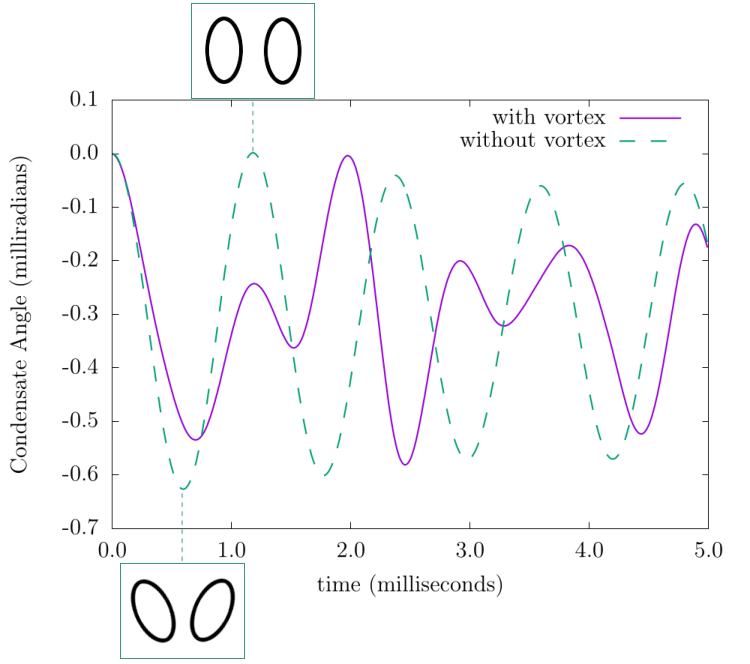
\includegraphics[width=0.75\textwidth]{data/3d/scissors_plot.pdf}
\label{fig:scissors}
\caption{\label{fig:scissors} Angle of the condensate axis after excitation of the toroidal scissors mode for an elliptic-toroidal BEC with a single vortex ring (purple, solid) and without a vortex present (cyan, dashed).
Depictions of two dimensional slices for the scissors mode without a vortex are shown in the insets.
Here, the scissors mode causes oscillation in and out towards the center of the system, and that two distinct frequencies are present in the curve for the condensate carrying a vortex ring. }
\end{figure}

Observing the presence of vortex rings in a three dimensional BEC is a difficult problem, as absorption spectroscopy usually only provides a picture of an integrated two-dimensional density.
However, due to the unique geometry of this system, one can identify whether vortex rings are present by exciting the scissors mode of the condensate \cite{cozzini2003, guery1999, marago2000}. 
For an elliptic-toroidal geometry ($\omega_z < \omega_r$), the scissors mode can be excited by modifying the external potential with a rotation in the $r-z$ plane,
\begin{equation}
        V = V_{\text{trap}}(r, \theta, z) -m\omega_0^2\alpha rz,
\end{equation}
where $\alpha = 2\epsilon\theta$ is a coefficient related to the tilting angle, $\epsilon$ is the deformation of the trap in the $r-z$ plane and $\theta$ is the angle at which the original trap was aligned at.
For a small initial angle of $\theta_0$ this change in the potential causes a BEC without rotation to oscillate back and forth in the trap with a frequency given by \cite{stringari2001}
\begin{equation}
        \omega_{\text{scissors}} = \sqrt{\omega_r^2+\omega_z^2}.
\end{equation}
If, however, this mode is excited for a BEC that contains a vortex line, the oscillation will be strongly influenced by the currents inside the condensate and two different frequencies ($\omega_+$ and $\omega_-$) appear in the oscillation~\cite{smith2004, zambelli1998, stringari2001}.
When the splitting frequency is small compared to the scissors mode frequency, it 
can be written as \cite{zambelli1998}
\begin{equation}
\omega_{+} - \omega_{-} = \frac{\langle l_z \rangle}{m\langle r^2 + z^2 \rangle},
\label{eqn:splitting}
\end{equation}
where $\langle l_z \rangle$ is the average angular momentum per particle.
Calculating these values for the system for $\omega_r = 4242$Hz, and $\omega_z = 2828$Hz then leads to $\omega_{\text{scissors}} = 5090$Hz, $\omega_{-} = 3765$Hz, and $\omega_{+} = 6415$Hz, which are very close to the values observed in the numerical simulations shown in Fig.~\ref{fig:scissors}.
However, one can also see from this figure that the oscillation is not perfect and seems to decay over time.
This is due to the above mentioned modification of the trapping potential by the artificial vector potential, which leads to a deviation from the perfect elliptical toroidal shape used in the derivation of Equation~\eqref{eqn:splitting}.

It is worth noting that this method cannot be used to detect a vortex ring inside a simply connected condensate, as in this situation the flow around the vortex line has no preferred direction.
However, in the toroidal shape, each radial slice can be seen as a two-dimensional elliptical BEC with a single vortex, and the system will therefore exhibit the scissors mode frequency as expected.
While in principle the excitation of the scissors mode can also be used to detect Abrikosov vortex-ring lattice, the fact that the inhomogeneous artificial magnetic field leads to an inhomogeneous vortex ring distribution will have an effect on the expected oscillation frequencies.

\section{Outlook}

In this application of the GPUE codebase, I have shown that it is possible to create and control vortex rings and ring-like vortex structures by using the artificial magnetic field generated by the optical nanofiber.
There is currently no other known method to generate the structures created by the linearly polarized modes, shown in Figure~\ref{fig:VortexRings}(b,c) and \ref{fig:HE21_3d}.
I have also shown that the scissors mode can be used to detect whether a vortex ring is present in an elliptic toroidal trap.
These fiber-generated structures could allow for experimental systems to study superfluid mechanisms, like the kelvin-mode cascade, superfluid turbulence, or reconnection events between superfluid vortex lines.
This might also be the first step in creating knotted vortex lines around an optical nanofiber; however, to generate these structures, the magnetic field must have a dependence on $\hat z$, which is not present in this model.

This project leaves several open fields of study for future work and future simulations with GPUE, including the study of dynamic field effects on vortex structures, the generation of vortex knots in superfluid systems with this device, and studies of vortex ring lattice movement in BEC systems.
For both of these cases, significant work must be performed both theoretically and computationally.

To generate vortex knots with this system, a magnetic field with $\hat z$ must be created.
Such fields might be possible with fiber Bragg gratings~\cite{hill1997} or other methods to change the evanescent profile of the fiber.
Such simulations would require FEM or FDTD simulations of the optical fiber, itself, which makes the problem an intricate engineering process of generating the right field with an optical nanofiber.
In addition, a z-dependent gauge field requires analysis of the other gauge field term, $\frac{p_z\mathbf{A}_z}{2}$, which is not considered in this work because the derivative along the $\hat z$ direction for the fiber field is 0.
This leads to interesting questions about how BEC systems behave in the presence of such artificial magnetic fields.

For the movement of dynamic vortex ring tangles generated with this system, vortex tracking methods in three-dimensions should be employed.
As described in Chapter~\ref{ch:gpu}, this is not a trivial task and I will discuss methods that could be used to do this in the outlook of this work, Chapter~\ref{ch:conclusion}.
It is also interesting to see what happens if the HE$_{21}$ vortex structures are evolved in real-time and whether scissors modes can be used to detect such vortex structures as well.
With a sharp magnetic field, it might also possible to create a phase separation along a vortex line for multicomponent condensate simulations, which could be an interesting area for future work.
